\documentclass[a4paper]{article}
\usepackage[utf8]{inputenc}
\usepackage[russian,english]{babel}
\usepackage[T2A]{fontenc}
\usepackage[left=10mm, top=20mm, right=18mm, bottom=15mm, footskip=10mm]{geometry}
\usepackage{indentfirst}
\usepackage{amsmath,amssymb}
\usepackage[italicdiff]{physics}
\usepackage{graphicx}
\graphicspath{{images/}}
\DeclareGraphicsExtensions{.pdf,.png,.jpg}
\usepackage{wrapfig}

\usepackage{caption}
\captionsetup[figure]{name=Рисунок}
\captionsetup[table]{name=Таблица}
  
\title{\underline{Отчет о выполненой лабораторной работе 1.1.4}}
\author{Воронин Денис, Б04-403}

\begin{document}
\maketitle
\textbf{Изучение статистических
закономерностей на примере измерения
фона космического излучения}

\section{Аннотация}
\textbf{Цель работы:} на примере статистики регистрации фоновых космических частиц изучить статистические закономерности однородного во времени случайного процесса;
проверить возможность описания исследуемого процесса статистическими законами 

\textbf{В работе используются:} счётчик Гейгера—Мюллера, компьютер с интерфейсом для 
связи со счётчиком, расчётная программа.


\section{Теоретические сведения}
\subsection{Оборудование}

\begin{wrapfigure}{R}{.3\textwidth}
\centering
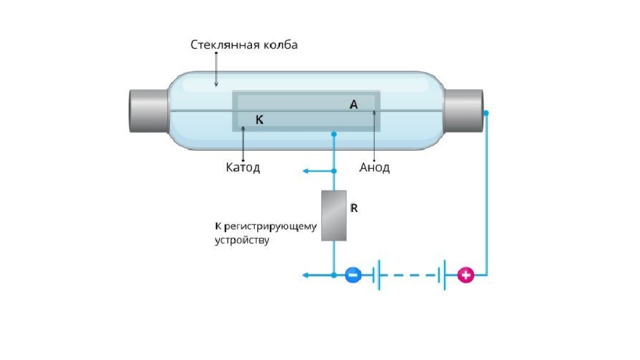
\includegraphics[width=80mm\textwidth]{img6.jpg}
\caption{Устройство счетчика}
\end{wrapfigure}

В данной работе для регистрации космического излучения используется счётчик Гейгера—Мюллера. Счётчик представляет собой наполненный газом металлический цилиндр с двумя электродами. Одним из электродов (катодом) служит сам корпус. Другим (анодом) является тонкая нить, натянутая вдоль оси цилиндрического корпуса. Необходимое напряжение (400 В) подаётся на счётчик от смонтированного вместе с ним блока питания через повышающий трансформатор. Радиоактивное излучение (космические частицы) ионизует молекулы газа, которым наполнен счётчик, а также выбивает электроны из его стенок. Образовавшиеся электроны, двигаясь в сильном электрическом ноле между электродами счётчика, соударяются с молекулами газа, выбивая из них новые — вторичные электроны. Ускоряясь полем, первичный и вторичные электроны снова ионизуют газ, и т.д. В результате образуется лавина электронов, и через счётчик протекает кратковременный импульс тока (разряд). Этот импульс и регистрируется электрической цепью установки, оцифровывается платой аналогово-цифрового преобразователя, и информация о нём через USB-интерфейс передаётся на компьютер.(рис.1) \par
Число зарегистрированных частиц за некоторое время зависит, вообще говоря, от размеров счётчика, положения и ориентации его в пространстве, от давления и состава газа и от материала стенок счётчика. Однако при фиксированном положении конкретного счётчика их число пропорционально 
средней интенсивности пронизывающего счётчик ионизирующего излучения. При постоянной фоновой интенсивности общее количество зарегистрированных частиц будет, конечно, пропорционально времени наблюдения t.


\subsection{Базовые погрешности}
Наиболее важной характеристикой является среднее число регистрируемых частиц в единицу времени. Если $n_{1}, n_{2}, ..., n_{N}$ - результаты N проведённых в одинаковых условиях измерений, можно вычислить выборочное среднее значение числа измерений:
\[\langle n \rangle = \frac{1}{N}\sum\limits_{i=1}^{N} n_{i}\]
Если продолжать проводить измерения, можно ожидать, что выборочное среднее будет стремиться к некоторому конечному пределу, который можно назвать «истинным» средним значением числа регистрируемых частиц. Втеории вероятностей оно называется «математическим ожиданием» случайной величины:
\[\overline{n} = \lim_{N \to \infty} \langle n \rangle\]
Количественно меру флуктуаций среднего значения от опыта к опыту принято измерять среднеквадратичным (или стандартным) отклонением $\sigma_{n}$
По определению, средний квадрат отклонения, называемый также дисперсией, равен:
\[\sigma_{n}^2 = \frac{1}{N}\sum\limits_{i=1}^{N} (n_{i} - \langle n \rangle)^2 = \langle (n_{i} - \langle n \rangle)^2 \rangle\]
Погрешность среднего значения $\langle n \rangle$ при независимых измерениях связана с погрешностью отдельного измерения формулой:
\[\sigma_{\langle n \rangle} = \frac{\sigma_{n}}{\sqrt{N}}\]
Таким образом, увеличивая количество измерений, среднее значение приближается к «истинному» n. При конечном N истинное среднее с высокой вероятностью лежит в интервале 
\[\overline{n} = \langle n \rangle \pm \frac{\sigma_{n}}{\sqrt{N}}\]

\subsection{Пуассоновский процесс}
Если события однородны во времени и каждое следующее событие не зависит от прошлого, то последовательность таких событий называют \textit{пуассоновский процессом}.\newline

\begin{figure}[t]
    \centering
    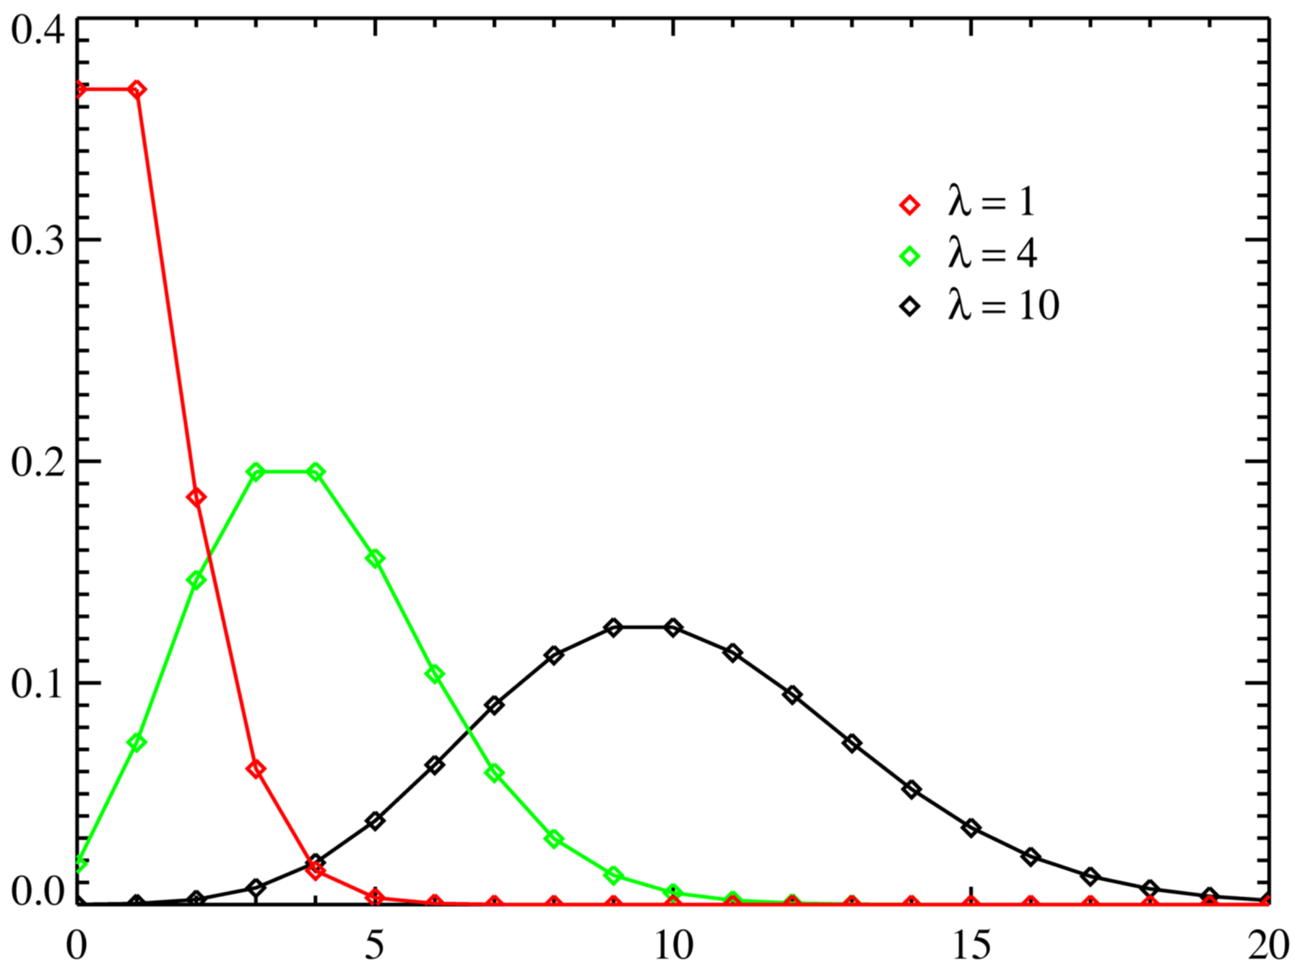
\includegraphics[width=0.6\textwidth]{paus.png}
    \caption{График распределения Пуассона}
\end{figure}

Вероятности $\omega_{n}$ того, что в эксперименте будет обнаружено n частиц, для распределения Пуассона имеют вид:
\[\omega_{n} =  \frac{\overline{n}^{n}}{n!} e^{-\overline{n}}\]
\newline
При больших $\overline{n} > 10$ график распределения (рис.2) стремиться к гладкой симметричной кривой, быстро убывающей к нулю при отдалении от центра.
\newline
Для пуассоновского процесса справедливо равенство:
\[\sigma = \sqrt{\overline{n}}\]
То есть среднеквадратичное отклонение равно корню из среднего. На практике можно ожидать приближённое равенство для выборочных значений:
\[\sigma_{n} \approx \sqrt{\langle n \rangle}\]

\section{Погрешность эксперимента}

Если подставить основное свойство распределения Пуассона в формулу погрешности среднего значения, то получится среднеквадратичная погрешность определения среднего:
\[\sigma_{\langle n \rangle} = \frac{\sigma_{n}}{\sqrt{N}} = \sqrt{\frac{\langle n \rangle}{N}}\]
Для относительного значения погрешности:
\[\varepsilon_{\langle n \rangle} = \frac{\sigma_{\langle n \rangle}}{\langle n \rangle} = \frac{1}{\sqrt{\langle n \rangle N}}\]

Таким образом, единственный способ увеличить точность опыта — увеличивать общее число регистрируемых частиц  $n_\Sigma$ за счёт увеличения совокупности времени измерений t. Например, для достижения точности измерений интенсивности фона в $\varepsilon = 1\%$ необходимо зарегистрировать в общей сложности сложности не менее $\frac{1}{0,01^{2}} = 10^{4}$ частиц.

\section{Обработка результатов}
\subsection{Вычисление погрешностей}

В данном эксперименте будут обработанны данные для 4х времен: $\tau = 10\text{с}, \tau = 20\text{с}, \tau = 40\text{с}, \tau = 80\text{с}$.



Вычислим среднее число срабатываний счетчика за 10с,20с,40с,80с:
\[\overline{n_{10}} = \frac{1}{10}\sum\limits_{i=1}^{10} n_{i} \approx 12,8\]
\[\overline{n_{20}} = \frac{1}{20}\sum\limits_{i=1}^{20} n_{i} \approx 25,7\]
\[\overline{n_{40}} = \frac{1}{40}\sum\limits_{i=1}^{40} n_{i} \approx 52,28\]
\[\overline{n_{80}} = \frac{1}{80}\sum\limits_{i=1}^{80} n_{i} \approx 104,7\]


Вычислим стандартное отклонение для 10с,20с,40с,80с:
\[\sigma_{n_{10}} = \sqrt{\frac{1}{10}\sum\limits_{i=1}^{10} (n_{i} - \overline{n_{10}})^2} \approx 4,04\]
\[\sigma_{n_{20}} = \sqrt{\frac{1}{20}\sum\limits_{i=1}^{20} (n_{i} - \overline{n_{20}})^2} \approx 6,41\]
\[\sigma_{n_{40}} = \sqrt{\frac{1}{40}\sum\limits_{i=1}^{40} (n_{i} - \overline{n_{40}})^2} \approx 6,96\]
\[\sigma_{n_{80}} = \sqrt{\frac{1}{50}\sum\limits_{i=1}^{80} (n_{i} - \overline{n_{80}})^2} \approx 8,26\]
Рассчитаем среднеквадратическое отклонение по свойству процесса Пуассона и сравним с стандартной:
\[\sigma_{n_{10}} = \sqrt{\overline{n_{10}}} \approx 3,58 \pm 4,04\]
\[\sigma_{n_{20}} = \sqrt{\overline{n_{20}}} \approx 5,07 \pm 6,41\]
\[\sigma_{n_{40}} = \sqrt{\overline{n_{40}}} \approx 7,23 \pm 6,96\]
\[\sigma_{n_{80}} = \sqrt{\overline{n_{40}}} \approx 10,23 \pm 8,26\]

Определим долю случаев, когда отклонения от среднего значения не превышают $\sigma_{n}$ и $2\sigma_{n}$ и сравним с теоретическими оценками - Таблица 8.
Рассчитаем погрешность среднего значения $\sigma_{\langle n \rangle} = \frac{\sigma_{n}}{\sqrt{N}}$:
\[\sigma_{\langle n_{10} \rangle} = \frac{\sigma_{n_{10}}}{\sqrt{400}} \approx 0,18\]
\[\sigma_{\langle n_{20} \rangle} = \frac{\sigma_{n_{20}}}{\sqrt{200}} \approx 0,36\]
\[\sigma_{\langle n_{40} \rangle} = \frac{\sigma_{n_{20}}}{\sqrt{100}} \approx 0,723\]
\[\sigma_{\langle n_{80} \rangle} = \frac{\sigma_{n_{20}}}{\sqrt{50}} \approx 1,45\]
Для каждого $\tau$ вычислим среднюю интенсивность регистрируемых частиц в секунду $\overline{j} = \frac{\overline{n}}{\tau}$ и её погрешность 
$\sigma_{j} = \frac{\sigma_{n}}{\tau}$:
\[\overline{j_{10}} = \frac{\overline{n_{10}}}{10} \approx 1,28\]
\[\sigma_{j_{10}} = \frac{\sigma_{\langle n_{10} \rangle}}{10} \approx 0,018\]
\[\overline{j_{10}} = \langle j_{10} \rangle \pm \sigma_{j_{10}} = 1,28 \pm 0,018 \]
\[\langle j_{20} \rangle = \frac{\overline{n_{20}}}{20} \approx 1,28\]
\[\sigma_{j_{20}} = \frac{\sigma_{\langle n_{20} \rangle}}{20} \approx 0,018\]
\[\overline{j_{20}} = \langle j_{20} \rangle \pm \sigma_{j_{20}} = 1,28 \pm 0,018 \]
\[\langle j_{40} \rangle = \frac{\overline{n_{40}}}{40} \approx 1,3\]
\[\sigma_{j_{40}} = \frac{\sigma_{\langle n_{40} \rangle}}{40} \approx 0,018\]
\[\overline{j_{40}} = \langle j_{40} \rangle \pm \sigma_{j_{40}} = 1,3 \pm 0,018 \]
\[\langle j_{80} \rangle = \frac{\overline{n_{80}}}{80} \approx 1,3\]
\[\sigma_{j_{80}} = \frac{\sigma_{\langle n_{80} \rangle}}{80} \approx 0,018\]
\[\overline{j_{80}} = \langle j_{80} \rangle \pm \sigma_{j_{80}} = 1,3 \pm 0,018 \]
Заметим, что средняя интенсивность регистрируемых частиц в секунду не зависит от величины интервала $\tau$ и числа точек N.

Обработаем данные из вышевычисленных и таблиц с данными и построим гистограммы зависимости долей случаев от их числа. Экспериментальные гистограммы (рисунки 3-6) с большой точностью согласуются с распределениями Пуассона. 


\subsection{Вывод}
На примере статистики регистрации фоновых космических частиц изучил статистические закономерности однородного во времени случайного процесса.Выяснил, что средняя интенсивность регистрируемых частиц в секунду не зависит от величины интервала $\tau$ и числа точек N. Исследовал Пуассоновский процесс и распределение Гаусса. \par



\newpage



\section{Данные, таблицы и гистограммы}
\begin{table}[!h]
\begin{center}
\begin{tabular}{|l|l|l|l|l|l|l|l|l|l|l|}
\hline
        & 1  & 2  & 3  & 4  & 5  & 6  & 7  & 8  & 9  & 10  \\ \hline
0       & 18 & 24 & 26 & 23 & 37 & 27 & 15 & 15 & 15 & 27 \\ \hline
10      & 15 & 20 & 33 & 34 & 27 & 31 & 32 & 28 & 23 & 27 \\ \hline
20      & 32 & 28 & 25 & 32 & 22 & 20 & 30 & 23 & 26 & 34 \\ \hline
30      & 20 & 27 & 35 & 24 & 24 &27 & 20 & 31 & 23 & 29 \\ \hline
40      & 30 & 29 & 27 & 22 & 24 & 28 & 21 & 39 & 29 & 33 \\ \hline
50      & 35 & 21 & 24 & 24 & 26 & 23 & 24 & 22 & 28 & 18 \\ \hline
60      & 24 & 27 & 36 & 24 & 29 & 28 & 22 & 40 & 26 & 16 \\ \hline
70      & 30 & 24 & 21 & 32 & 26 & 20 & 26 & 31 & 31 & 28 \\ \hline
80      & 24 & 29 & 25 & 25 & 26 & 20 & 32 & 21 & 22 & 38 \\ \hline
90      & 29 & 26 & 28 & 22 & 30 & 24 & 27 & 31 & 32 & 36 \\ \hline
100     & 25 & 25 & 29 & 27 & 23 & 30 & 28 & 28 & 16 & 28 \\ \hline
110     & 27 & 24 & 26 & 26 & 27 & 33 & 23 & 21 & 23 & 25 \\ \hline
120     & 28 & 31 & 37 & 27 & 34 & 24 & 28 & 33 & 30 & 23 \\ \hline
130     & 29 & 30 & 27 & 23 & 27 & 24 & 23 & 23 & 31 & 32 \\ \hline
140     & 27 & 20 & 23 & 28 & 25 & 24 & 23 & 26 & 23 & 23 \\ \hline
150     & 23 & 26 & 28 & 27 & 29 & 22 & 25 & 34 & 24 & 30 \\ \hline
160     & 28 & 21 & 33 & 23 & 22 & 28 & 31 & 22 & 34 & 29 \\ \hline
170     & 25 & 32 & 16 & 31 & 19 & 32 & 32 & 24 & 30 & 19 \\ \hline
180     & 33 & 24 & 27 & 27 & 22 & 22 & 33 & 29 & 18 & 21 \\ \hline
190     & 25 & 31 & 30 & 24 & 19 & 24 & 29 & 30 & 31 & 26 \\ \hline
\end{tabular}
\caption{Число срабатываний счетчика за $\tau = 20$ с}
\end{center}
\end{table}

\begin{table}[!h]
\begin{center}
\begin{tabular}{|l|l|l|l|l|l|l|l|l|l|l|}
\hline
   & 1  & 2  & 3  & 4  & 5  & 6  & 7  & 8  & 9  & 10 \\ \hline
0  & 42 & 49 & 64 & 30 & 42 & 53 & 61 & 63 & 51 & 59 \\ \hline
10 & 53 & 54 & 50 & 49 & 54 & 62 & 48 & 62 & 51 & 52 \\ \hline
20 & 44 & 63 & 55 & 50 & 49 & 44 & 49 & 51 & 49 & 53 \\ \hline
30 & 51 & 60 & 57 & 62 & 42 & 54 & 53 & 46 & 57 & 59 \\ \hline
40 & 53 & 50 & 46 & 53 & 60 & 55 & 50 & 54 & 58 & 68 \\ \hline
50 & 50 & 56 & 53 & 56 & 44 & 51 & 52 & 60 & 44 & 48 \\ \hline
60 & 59 & 64 & 58 & 61 & 53 & 59 & 50 & 51 & 46 & 63 \\ \hline
70 & 47 & 51 & 49 & 49 & 46 & 49 & 55 & 51 & 59 & 54 \\ \hline
80 & 49 & 56 & 50 & 53 & 63 & 57 & 47 & 51 & 56 & 49 \\ \hline
90 & 57 & 54 & 44 & 62 & 39 & 56 & 54 & 43 & 59 & 57 \\ \hline
\end{tabular}
\caption{Число срабатываний счетчика за $\tau = 40$ с}
\end{center}
\end{table}

\begin{table}[!h]
\begin{center}
\begin{tabular}{|l|l|l|l|l|l|l|l|l|l|l|}
\hline
   & 1  & 2  & 3  & 4  & 5  & 6  & 7  & 8  & 9  & 10 \\ \hline
0  & 91 & 94 & 95 & 124 & 110 & 107 & 99 & 116 & 110 & 103 \\ \hline
10 & 107 & 105 & 93 & 100 & 102 & 106 & 113 & 108 & 108 & 100 \\ \hline
20 & 116 & 114 & 104 & 94 & 101 & 98 & 92 & 116 & 111 & 110 \\ \hline
30 & 96 & 91 & 111 & 104 & 116 & 99 & 95 & 122 & 100 & 107 \\ \hline
40 & 112 & 109 & 101 & 102 & 95 & 114 & 112 & 109 & 98 & 101 \\ \hline
\end{tabular}
\caption{Число срабатываний счетчика за $\tau = 80$ с}
\end{center}
\end{table}


\begin{table}[!h]
\begin{center}
\begin{tabular}{|l|l|}
\hline
Число импульсов, $n_{i}$ & Доля случаев, $\omega_{n}$ \\ \hline
4                        & 0.003                     \\ \hline
5                        & 0.003                     \\ \hline
6                        & 0.023                     \\ \hline
7                        & 0.033                     \\ \hline
8                        & 0.030                      \\ \hline
9                        & 0.073                     \\ \hline
10                       & 0.083                     \\ \hline
11                       & 0.123                      \\ \hline
12                       & 0.093                      \\ \hline
13                       & 0.113                       \\ \hline
14                       & 0.090                    \\ \hline
15                       & 0.078                     \\ \hline
16                       & 0.088                     \\ \hline
17                       & 0.063                       \\ \hline
18                       & 0.038                     \\ \hline
19                       & 0.028                     \\ \hline
20                       & 0.010                       \\ \hline
21                       & 0.015                      \\ \hline
22                       & 0.005                      \\ \hline
23                       & 0.008                      \\ \hline
24                       & 0.003                      \\ \hline
25                       & 0.005                     \\ \hline
\end{tabular}
\caption{Данные для гистограммы распределение при $\tau = 10$ с}
\end{center}
\end{table}


\begin{table}[!h]
\begin{center}
\begin{tabular}{|l|l|}
\hline
Число импульсов, $n_{i}$ & Доля случаев, $\omega_{n}$ \\ \hline
15                       & 0.020                      \\ \hline
16                       & 0.010                      \\ \hline
17                       & 0.005                       \\ \hline
18                       & 0.025                      \\ \hline
19                       & 0.025                       \\ \hline
20                       & 0.055                       \\ \hline
21                       & 0.035                       \\ \hline
22                       & 0.055                       \\ \hline
23                       & 0.070                      \\ \hline
24                       & 0.090                       \\ \hline
25                       & 0.050                      \\ \hline
26                       & 0.075                       \\ \hline
27                       & 0.110                       \\ \hline
28                       & 0.090                       \\ \hline
39                       & 0.035                       \\ \hline
30                       & 0.035                      \\ \hline
31                       & 0.075                       \\ \hline
32                       & 0.030                      \\ \hline
33                       & 0.020                      \\ \hline
34                       & 0.030                       \\ \hline
35                       & 0.020                       \\ \hline
36                       & 0.015                       \\ \hline
37                       & 0.020                      \\ \hline
38                       & 0.005                      \\ \hline
\end{tabular}
\caption{Данные для гистограммы распределение при $\tau = 20$ с}
\end{center}
\end{table}

\begin{table}[!h]
\begin{center}
\begin{tabular}{|l|l|}
\hline
Число импульсов, $n_{i}$ & Доля случаев, $\omega_{n}$ \\\hline
30                       & 0.010                       \\\hline
38                       & 0.020                       \\\hline
42                       & 0.040                       \\\hline
43                       & 0.010                       \\\hline
44                       & 0.020                       \\\hline
45                       & 0.050                      \\\hline
46                       & 0.020                      \\\hline
47                       & 0.040                      \\\hline
48                       & 0.050                      \\\hline
49                       & 0.090                      \\\hline
50                       & 0.050                      \\\hline
51                       & 0.050                      \\\hline
52                       & 0.060                      \\\hline
53                       & 0.090                      \\\hline
54                       & 0.040                      \\\hline
55                       & 0.060                     \\\hline
56                       & 0.050                      \\\hline
57                       & 0.050                      \\\hline
58                       & 0.020                      \\\hline
59                       & 0.040                      \\\hline
61                       & 0.010                      \\\hline
62                       & 0.030                      \\\hline
63                       & 0.030                      \\\hline
64                       & 0.050                      \\\hline
65                       & 0.010                      \\\hline
66                       & 0.010                      \\\hline
\end{tabular}
\caption{Данные для гистограммы распределение при $\tau = 40$ с}
\end{center}
\end{table}

\begin{table}[!h]
\begin{center}
\begin{tabular}{|l|l|}
\hline
Число импульсов, $n_{i}$ & Доля случаев, $\omega_{n}$ \\\hline
91                       & 0.040                       \\\hline
92                       & 0.040                       \\\hline
93                       & 0.020                       \\\hline
94                       & 0.040                       \\\hline
95                       & 0.060                       \\\hline
96                       & 0.020                      \\\hline
98                       & 0.020                      \\\hline
99                       & 0.040                      \\\hline
100                       & 0.060                      \\\hline
101                      & 0.040                      \\\hline
102                      & 0.060                      \\\hline
103                      & 0.020                      \\\hline
104                      & 0.040                      \\\hline
105                      & 0.090                      \\\hline
106                      & 0.020                      \\\hline
107                      & 0.020                     \\\hline
108                      & 0.060                      \\\hline
109                      & 0.060                      \\\hline
110                      & 0.020                      \\\hline
111                      & 0.020                      \\\hline
112                      & 0.060                      \\\hline
113                      & 0.040                      \\\hline
114                      & 0.040                      \\\hline
116                      & 0.080                     \\\hline
122                      & 0.020                      \\\hline
124                      & 0.0200                      \\\hline

\end{tabular}
\caption{Данные для гистограммы распределение при $\tau = 80$ с}
\end{center}
\end{table}


\begin{table}[!h]
\begin{center}
\begin{tabular}{|l|l|}
\hline
Число импульсов, $n_{i}$ & Доля случаев при распределении Пуассона, $\omega_{n}$ \\ \hline
4                       & 0.003                                                                                 \\ \hline
5                       & 0.008                                                                                  \\ \hline
6                       & 0.017                                                                                  \\ \hline
7                       & 0.031                                                                                 \\ \hline
8                       & 0.049                                                                                  \\ \hline
9                       & 0.070                                                                                  \\ \hline
10                       & 0.090                                                                                  \\ \hline
11                       & 0.105                                                                                  \\ \hline
12                       & 0.112                                                                                  \\ \hline
13                       & 0.110                                                                                  \\ \hline
14                       & 0.100                                                                                  \\ \hline
15                       & 0.086                                                                                  \\ \hline
16                       & 0.069                                                                                  \\ \hline
17                       & 0.052                                                                                  \\ \hline
18                       & 0.037                                                                                  \\ \hline
19                       & 0.025                                                                                 \\ \hline
20                       & 0.016                                                                                 \\ \hline
21                       & 0.010                                                                                 \\ \hline
22                       & 0.006                                                                                   \\ \hline
23                       & 0.003                                                                                 \\ \hline
24                       & 0.002                                                                                 \\ \hline
25                       & 0.001                                                                                 \\ \hline

\end{tabular}
\caption{Данные для гистограммы распределение Пуассона при $\tau = 10$ с}
\end{center}
\end{table}



\begin{table}[!h]
\begin{center}
\begin{tabular}{|l|l|l|l|}
\hline
Ошибка                             & Число случаев & Доля случаев, \% & Теоретическая оценка \\ \hline
$\pm\sigma_{n_{20}} = \pm 6,41$    & 145           & 72,5             & 68                   \\ \hline
$\pm 2\sigma_{n_{20}} = \pm 12,82$  & 188           & 94               & 95                   \\ \hline
$\pm 3\sigma_{n_{20}} = \pm 19,23$ & 200           & 100              & 99                   \\ \hline
$\pm\sigma_{n_{40}} = \pm 6,96$    & 67            & 67               & 68                   \\ \hline
$\pm 2\sigma_{n_{40}} = \pm 13,92$ & 97            & 97               & 95                   \\ \hline
$\pm 3\sigma_{n_{40}} = \pm 20,88$ & 100           & 100              & 99                   \\ \hline
$\pm\sigma_{n_{80}} = \pm 8,26$    & 37            & 74               & 75                   \\ \hline
$\pm 2\sigma_{n_{80}} = \pm 16,52$ & 48            & 96               & 95                   \\ \hline
$\pm 3\sigma_{n_{80}} = \pm 24,78$ & 50           & 100              & 99                   \\ \hline
\end{tabular}
\caption{Оценка распределения доли случаев}
\end{center}
\end{table}

\begin{figure}[t]
    \centering
    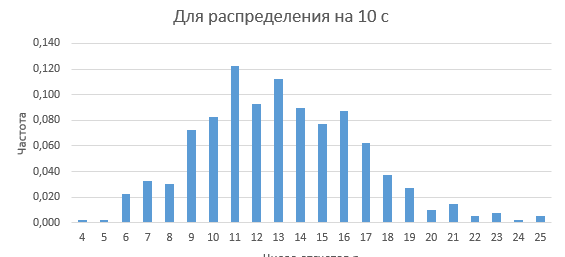
\includegraphics[width=140mm\textwidth]{10c.PNG}
    \caption{Гистограмма при $\tau = 10$}
\end{figure}

\begin{figure}[t]
    \centering
    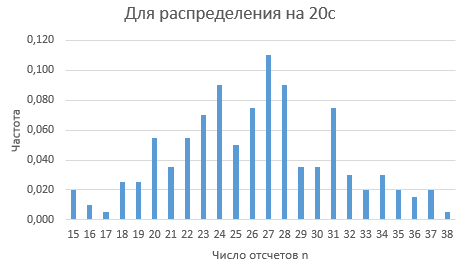
\includegraphics[width=140mm\textwidth]{20c.PNG}
    \caption{Гистограмма при $\tau = 20$}
\end{figure}

\begin{figure}[t]
    \centering
    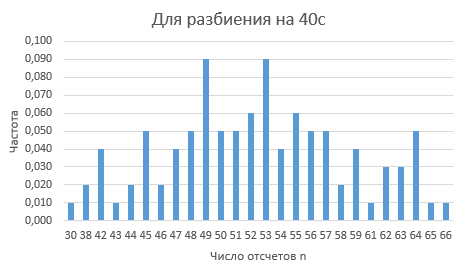
\includegraphics[width=140mm\textwidth]{40c.PNG}
    \caption{Гистограмма при $\tau = 40$}
\end{figure}

\begin{figure}[t]
    \centering
    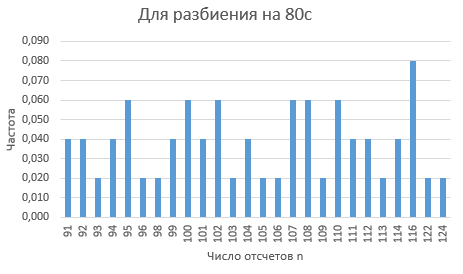
\includegraphics[width=140mm\textwidth]{80c.PNG}
    \caption{Гистограмма при $\tau = 80$}
\end{figure}

\begin{figure}[t]
    \centering
    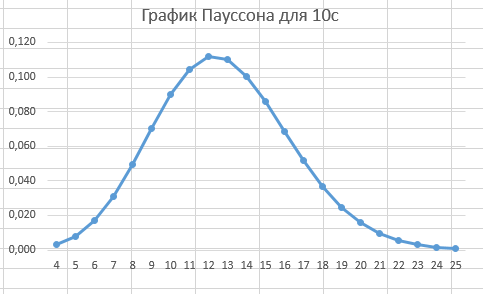
\includegraphics[width=140mm\textwidth]{paus10.PNG}
    \caption{График Пауссона для  $\tau = 10$}
\end{figure}

\begin{figure}[t]
    \centering
    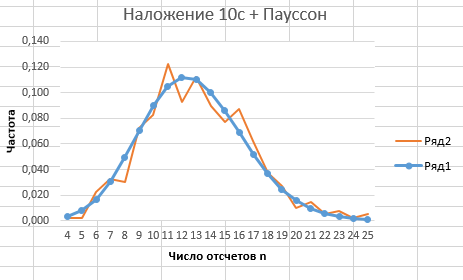
\includegraphics[width=140mm\textwidth]{pausnal_10c.PNG}
    \caption{Наложение Пауссона и экспериментальной гистограммы для  $\tau = 10$}
\end{figure}

\end{document}
